\section{实验任务与场地}
\subsection{任务要求与验收口径}
依据课程《第五--六章：基于视觉与 AI 定位的多机协同控制实验》\cite{course}，系统同时包含人形机器人搬运和多车跟随两项任务。TonyPi 从指定位置抱起目标物体，在障碍通道中至少完成两个转角（左右转各至少一次），到达终点后放下物体；TurtleBot2 保持跟随并在终点区域停靠。课程总体评价由现场竞赛与方案、源码报告构成，权重分别为80\%和20\%。手册中的任务平台数量写为3--4台 TurtleBot2，详细评分表按四台、四种方式设置；本报告为四种方式保留独立章节，实际参赛车辆与方式认定须由全队和教师确认。

\begin{table}[H]\centering\small
\caption{任务要求与对应记录}
\begin{tabularx}{\linewidth}{p{30mm}YY}\toprule
要求 & 系统对应内容 & 应提交的证据\\\midrule
抱持、转弯与放置 & 抓取动作、上肢锁定、A左转/B右转/C停止 & 连续视频、动作文件版本、决策日志\\
不接触障碍物 & 人形路线约束；TurtleBot代价地图与门控 & 接触次数、障碍位置、最小间距实测\\
保持跟随目标 & 标记身份、目标时效检查、失效处置 & 丢失次数、持续时间、重捕获记录\\
多种独立方式 & 四组分别说明观测来源和控制链 & 各组实现、接口及现场运行证据\\
协同到达终点 & 任务状态、各车停靠条件 & 全队同场运行记录与到达时间\\\bottomrule
\end{tabularx}\end{table}

表中的要求需要通过不同证据分别闭合：控制日志用于核对决策，连续视频用于确认持物、碰撞和最终停靠。只有软件状态结束而缺少现场记录时，不能据此判定整项比赛任务完成。


\subsection{场地与感知约束}
现场使用灰色地板及相对连续的灰色挡板构成通道，路线包含直行、左转、直行、右转和终点区域。地板接缝、胶带及其他地面标识均视为无关背景，不能作为路线识别标准。目标物块由早期蓝色调整为红色；抱持后物块可能遮挡画面下部，因此抓取确认与前方导航需要分别配置观察区域或头部姿态。

黄色雪糕筒可作为早期道路居中方案的终点候选；最新标记路线以固定标记 C 的距离触发停止。两种终点条件属于不同程序配置，不应在同一次实验记录中混写。图\ref{fig:route}仅表达路径拓扑，方向和长度以现场测量为准。
\begin{figure}[H]\centering
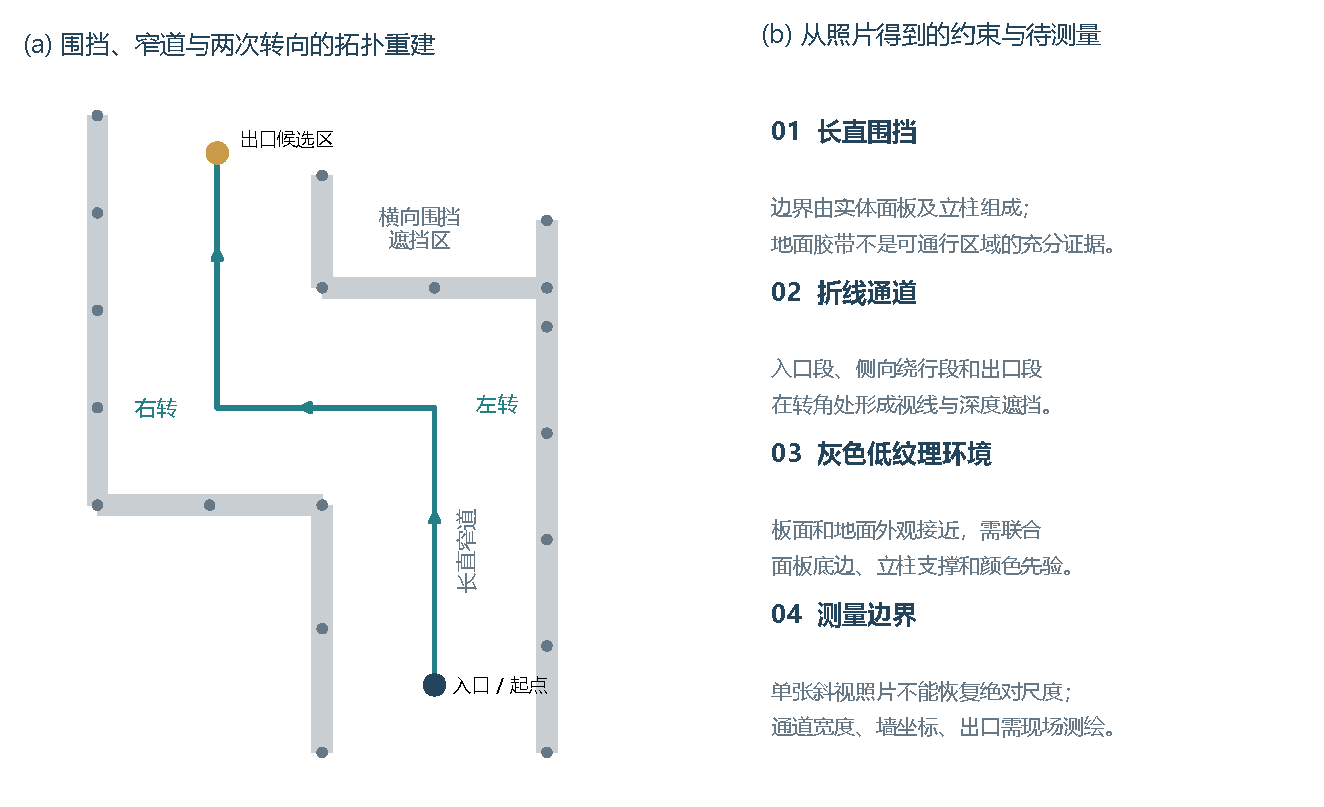
\includegraphics[width=.95\linewidth]{figures/analysis/arena.pdf}
\caption{路线拓扑示意；不按比例绘制，地面标识不参与定位}\label{fig:route}
\end{figure}

路线拓扑图用于说明 A/B/C 阶段与转向次序，不能代替场地测绘。拓扑上相邻的路段在相机视野中可能被围挡隔开，因此到达当前标记后仍需单独执行转角搜索。下面的实景照片补充展示围挡高度、通道边界与遮挡关系，使路线抽象与实际环境相互对应。

\begin{figure}[H]\centering
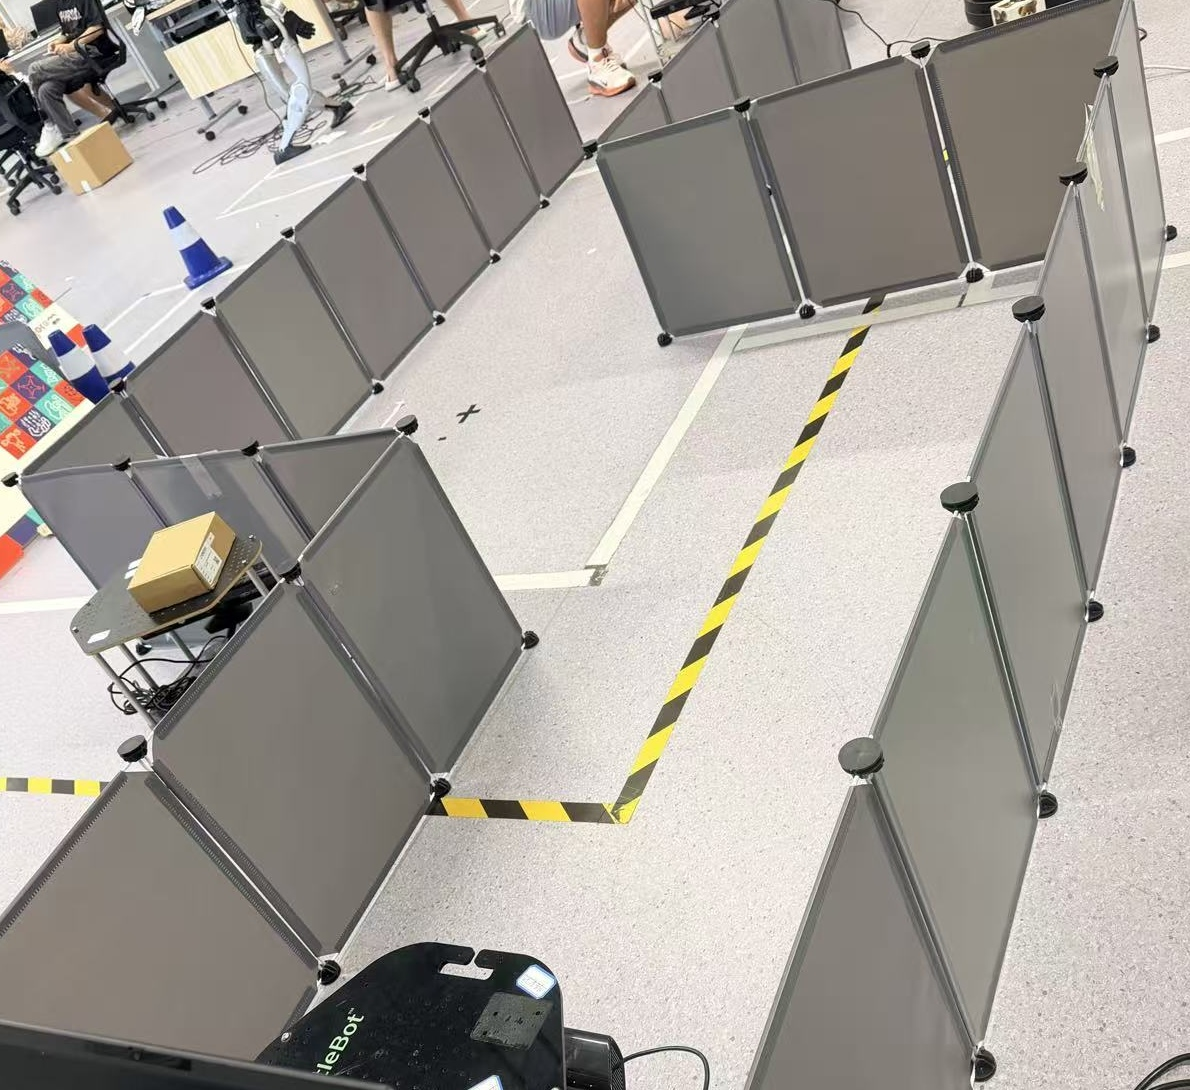
\includegraphics[width=.72\linewidth,height=.32\textheight,keepaspectratio]{figures/site/corridor_focus.jpg}
\caption{灰色挡板通道实景（裁去无关前景，原图保留）。连续围挡形成包含转角与视线遮挡的狭窄通道，近端可见 TurtleBot2 平台。照片由实验小组提供，仅用于说明现场结构，不据此恢复绝对尺度。}\label{fig:site-photo}
\end{figure}

实景中连续灰色挡板限制了跨路段观察，转角前后的目标可见性会明显变化。这解释了人形控制采用“当前标记抵近—搜索下一标记”的分段逻辑，也说明移动底盘即使获得目标位置，仍需结合地图和实时扫描检查通行条件。照片中的地面胶带仅用于现场布置说明，不作为视觉导航输入。

